\section{Marco Teorico} 

\begin{itemize}
\subsection{ Docker:}
	\item Tener un docker que provea el gestor de base de datos es muy útil porque se reducen tiempos de instalación y configuración y en caso de tener un error muy grave en la configuración es tan sencillo resolverlo como borrar el contenedor y crear uno nuevo.
          \item Los contenedores funcionan bien para desarrollo y tal vez algunos ambientes de evaluación para el cliente, pero para ambientes productivos para nada se recomiendan, en estos casos siempre será lo mejor que se cuente con una base de datos instalada en el servidor.
         \item Sirven para desplegar aplicaciones en un entorno virtual aislado, pero sin el overhead de tener un Sistema Operativo (SO) nuevo como se tiene en una Virtual Machine (VM).

\subsection{Oracle Database en Docker:}
	\item Los productos de Oracle son compatibles con Docker si el sistema operativo del host es Oracle Linux 7, pero no necesita usar un host OL7 para que esto funcione. Puedes ver cómo instalar Docker en OL7 .
	\item Usar imágenes de Oracle Container Registry o de Docker Store tiene la ventaja que los binarios de instalación vienen incluidos, lo que no es permitido por licencia en el resto de las distribuciones. 
\subsection{Referencias de cómo usar Oracle con Docker en Linux Y  en Windows:}
	\item Docker en Windows 10:
	\item Para usar la versión completa es necesario habilitar Microsoft Hyper-V, lo que implica deshabilitar la virtualización por hardware de nuestro PC. Si estamos usando VirtualBox en el mismo host, con este cambio deja de funcionar.
Docker Toolbox no tiene esta restricción, aunque se mantiene como una versión antigua (Legacy), y Docker recomienda usar la versión completa.Otra diferencia de Docker Toolbox es que necesita una VM VirtualBox para ejecutar. Esta VM se crea de forma automática al usar Toolbox, de nombre default, y se usa como host para los containers que creemos.
 \subsection{Construir la imagen:}
	\item La compilación espera el siguiente sistema de archivos. Tendrá que descargar la base de datos Oracle 19c y el software APEX usted mismo y colocarlo en el directorio "software".
                     \begin{figure}[H]
		\begin{center}
		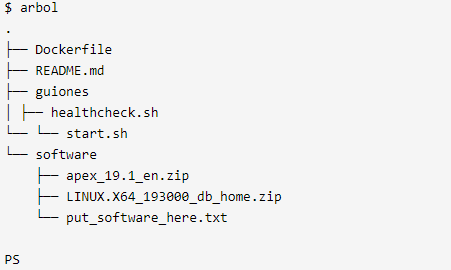
\includegraphics[width=8cm]{./Imagenes/100}
		\end{center}
		\end{figure}
	

\end{itemize}







